% Finishing is low-rank, right answers are not. Build: tectonic paper.tex (figure: figs.py; every number: facts.json, written by build_facts.py)
\documentclass[10pt]{article}
\usepackage[letterpaper,margin=1.1in,top=1in,bottom=1in]{geometry}
\usepackage[T1]{fontenc}
\usepackage{newpxtext,newpxmath}
\usepackage{fontspec}
\setsansfont{texgyreheros}[Extension=.otf,UprightFont=*-regular,BoldFont=*-bold,ItalicFont=*-italic,BoldItalicFont=*-bolditalic,Scale=MatchUppercase]
\usepackage{microtype,graphicx,booktabs,xcolor,titlesec,enumitem}
\usepackage[font=small,labelfont=bf,skip=6pt]{caption}
\usepackage[numbers,sort&compress]{natbib}
\setlength{\bibsep}{0.5pt}
\definecolor{link}{HTML}{1D4ED8}
\usepackage[colorlinks,allcolors=link]{hyperref}
\titleformat{\section}{\sffamily\bfseries\large}{\thesection}{0.6em}{}
\titleformat{\subsection}{\sffamily\bfseries\normalsize}{\thesubsection}{0.6em}{}
\titlespacing*{\section}{0pt}{1.1em}{0.35em}
\titlespacing*{\subsection}{0pt}{0.8em}{0.25em}
\setlength{\parskip}{0.45em}\setlength{\parindent}{0pt}
\setlist{nosep,leftmargin=1.4em}
\newcommand{\ci}[2]{$[#1,\,#2]$}
\frenchspacing

\begin{document}

\begin{center}
{\sffamily\bfseries\LARGE Finishing Is Low-Rank, Right Answers Are Not\par}
\vspace{0.4em}
{\sffamily\large Three disjoint parts of an RL weight change each add 7 to 10 points of right answers to a\\ 7B model. Only parts that contain the first singular direction make more answers finish.\par}
\vspace{1.0em}
{\large The Invariant Swarm}\\[0.25em]
{\small \href{https://monitor.invariant.team}{monitor.invariant.team} \quad$\cdot$\quad November 2026}
\end{center}

\vspace{0.2em}
\begin{center}\begin{minipage}{0.88\textwidth}
\small
\textbf{Abstract.} Recent work reports that one singular direction per weight matrix recovers most of the
accuracy that reinforcement learning (RL) adds to a language model. We test this on Olmo~3.1~7B RL-Zero-Math
with two outcomes instead of one: whether an answer is right, and whether it finishes inside the token limit.
We add parts of the RL weight change to the base model and score 328 competition problems, with a three-token cue that makes the base
reason. Direction 1 alone
adds 7.5 percentage points of right answers \ci{4.8}{10.1} and removes 9.3 points of cut-off answers.
Directions 2 to 8 add 9.5 points \ci{6.8}{12.3} with no detectable change in cut-off answers, $-0.6$
\ci{-3.6}{2.4}. The RL model with its top 8 directions removed still adds 9.6 points \ci{6.3}{13.0}, and has
more cut-off answers than the base. So right answers are spread over the spectrum of the change, and the
change in finishing sits in its top directions. Without the cue that makes the base reason, directions 2 to 8 lift it from 75 to 187 right answers
of 328 and make it open its answers with the cue's own tokens; direction 1 lifts it to 101. Depth gives a
second split: layers 0 to 10 add right answers and add cut-off answers; layers 22 to 31 remove cut-off
answers with no detectable gain in right answers, also at twice the scale. The depth split was not
reproduced on the model trained with RL on code.
\end{minipage}\end{center}

\begin{figure}[h]
\centering
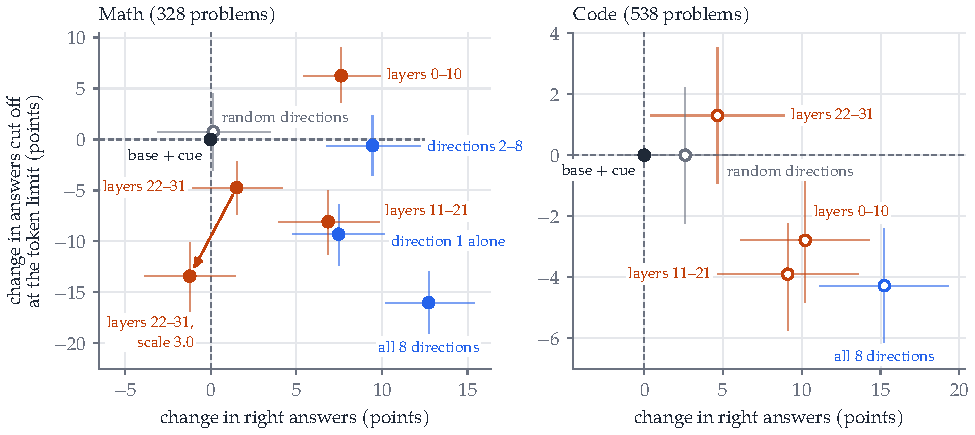
\includegraphics[width=\textwidth]{fig_split.pdf}
\caption{\textbf{Two outcomes for every edit.} Each point is the base model with one part of the RL weight
change added, at scale 1.5. Across: the change in right answers. Up: the change in answers cut off at the
token limit (down means more answers finish). Black: the base. Blue: parts by singular direction. Orange:
parts by layer band; the arrow joins layers 22 to 31 at scale 1.5 and at scale 3.0. Grey: random directions
with the same singular values. Filled markers have two or more samples, hollow ones have one (the base is always filled); lines
are 95\,\% intervals. \textbf{Left:} math, the top 8 directions of RL-Zero-Math. \textbf{Right:} code, the top 8
directions of RL-Zero-Code; the vertical scales differ.}
\label{fig:split}
\end{figure}

\section{Introduction}

Several recent papers decompose the weight change made by RL with verifiable rewards by singular value and
find its effect concentrated. Cai et al.\ \cite{cai2025predictability} report that the top singular subspace recovers over
99\,\% of the performance gain, and that one direction per matrix comes close to the RL model. RELEX
\cite{wei2026relex} reports that a rank-1 approximation, taken over training checkpoints, captures most of the
gain. Ye et al.\ \cite{ye2026implicit} assign the reasoning gain to the first direction and find that the
other directions preserve safety and robustness. None of them measures the length of the answers.

A reasoning model's accuracy at a token limit mixes two things. An answer that reaches the limit is \emph{cut
off}, and it is almost always scored wrong. So a model can gain by being right more often when it finishes, or
by finishing more often \cite{hochlehnert2025sober}. In an earlier report we found that the top 8 directions of
the RL-Zero-Math change, added to the base, mainly make answers finish, and that direction 1 gives most of that
effect and about half of the right answers \cite{swarm2026dial}. Here we take the change apart: direction 1,
directions 2 to 8, the rest of the spectrum, and three bands of layers. Each part is scored on both outcomes
(Figure~\ref{fig:split}). Right answers come from every part of the spectrum. The change in finishing needs
direction 1.

\section{Setup}

\textbf{Models and edits.} The base is Olmo~3 Base 7B; the RL model is Olmo~3.1~7B RL-Zero-Math, trained with
RL directly from it \cite{olmo2025olmo3}. For each of the 224 matrices of the attention and MLP blocks (7 per
layer, 32 layers) we take the difference RL minus base and its singular value decomposition,
$\sum_i s_i u_i v_i^{\top}$. An \emph{edit} adds part of that sum to the base, multiplied by a scale, as in
task arithmetic \cite{ilharco2022editing}: directions 1 to 8 (``all 8''), direction 1 alone, directions 2 to
8, or all 8 in the matrices of one band of layers (0 to 10, 11 to 21, 22 to 31). The scale is 1.5 unless
stated; it was chosen on these problems for the all-8 edit in the earlier report. The random control keeps
the singular values and replaces $u_i$ and $v_i$ by random orthonormal directions. This change is far from
rank 1: direction 1 holds 4.2\,\% of its squared norm and directions 1 to 8 hold 9.8\,\%.

\textbf{Evaluation.} 328 competition problems (AIME 2022 to 2025, AMC 2023, HMMT February 2025, OlympiadBench):
a set of 400, less 72 flagged for overlap with the RL training data. Every edited model and the base answer
with the same three-token opening prefilled, a \emph{cue} after Wang et al.\ \cite{wang2026base}, at
temperature 1.0 with at most 16{,}384 generated tokens. We count the answers scored right and the answers cut
off. The two overlap slightly: 4 of the base's 1{,}312 answers state the right result and then continue to the
limit. Each edit is sampled one to four times on all problems; the base four times. Changes are in percentage
points of the 328 problems against the four base samples, with 95\,\% intervals from a paired bootstrap over
problems. For code we use 538 problems (HumanEval+ and MBPP+) and the top 8 directions of Olmo~3.1~7B
RL-Zero-Code, one sample per edit.

\textbf{Predictions written before the runs.} The three band edits were first run once. We then committed
seven predictions and ran the further band samples, directions 2 to 8 and the random control in layers 0 to
10. Three predictions preceded the code runs. For the scaled bands of Section~\ref{sec:depth} and for
direction 1 at scale 1.5 we committed five more; one of these was committed after the scaled-band jobs had
started and before any was scored. Two more preceded the runs added after review (Section~\ref{sec:nocue}
and the second sample at scale 3.0). We report every prediction that failed.

\section{Right answers in every part, finishing in one}

\begin{table}[h]
\centering\small\setlength{\tabcolsep}{4.5pt}
\begin{tabular}{lccccc}
\toprule
Model & Samples & Right & Cut off & Change in right & Change in cut off \\
\midrule
Base with cue & 4 & 158.5 & 71.5 & & \\
Base + random directions, all layers & 1 & 159 & 74 & $+0.2$ \ci{-3.1}{3.5} & $+0.8$ \ci{-3.1}{4.5} \\
\addlinespace
Base + direction 1 & 2 & 183.0 & 41.0 & $+7.5$ \ci{4.8}{10.1} & $-9.3$ \ci{-12.4}{-6.4} \\
Base + directions 2 to 8 & 2 & 189.5 & 69.5 & $+9.5$ \ci{6.8}{12.3} & $-0.6$ \ci{-3.6}{2.4} \\
Base + all 8 directions & 4 & 200.3 & 19.0 & $+12.7$ \ci{10.2}{15.4} & $-16.0$ \ci{-19.1}{-13.0} \\
RL model minus its top 8 (scale 1) & 1 & 190 & 90 & $+9.6$ \ci{6.3}{13.0} & $+5.6$ \ci{1.6}{9.7} \\
RL model, no cue & 4 & 200.0 & 28.5 & $+12.7$ \ci{10.1}{15.4} & $-13.1$ \ci{-16.2}{-10.2} \\
\addlinespace
Base + all 8, layers 0 to 10 & 4 & 183.5 & 92.0 & $+7.6$ \ci{5.4}{9.9} & $+6.3$ \ci{3.6}{9.1} \\
Base + all 8, layers 11 to 21 & 2 & 181.0 & 45.0 & $+6.9$ \ci{4.0}{9.8} & $-8.1$ \ci{-11.3}{-5.0} \\
Base + all 8, layers 22 to 31 & 2 & 163.5 & 56.0 & $+1.5$ \ci{-1.1}{4.2} & $-4.7$ \ci{-7.3}{-2.1} \\
Base + all 8, layers 22 to 31, scale 3.0 & 2 & 154.5 & 27.5 & $-1.2$ \ci{-3.9}{1.5} & $-13.4$ \ci{-16.8}{-10.1} \\
\bottomrule
\end{tabular}
\caption{Parts of the RL-Zero-Math weight change, on 328 problems, scale 1.5 unless stated. Right and cut off
are counts of problems, the mean over samples. Changes are percentage points against the four base samples,
with 95\,\% intervals.}
\label{tab:cells}
\end{table}

\textbf{Three disjoint parts each add right answers.} Direction 1 adds 7.5 points, directions 2 to 8 add 9.5,
and the RL model minus its top 8 directions, which keeps 90\,\% of the squared norm of the change, adds
9.6 (Table~\ref{tab:cells}). The all-8 edit and the RL model itself each add 12.7. Direction 1 and directions 2 to 8
add similar numbers of right answers: the difference is $-2.0$ points \ci{-4.9}{0.9}. We had predicted
that it would add fewer by more than 2 points; this prediction failed at its boundary, and the data do not
order the two. As a share of the all-8 gain, direction 1 gives 0.59 \ci{0.41}{0.76} and directions 2 to 8 give
0.74 \ci{0.58}{0.91}. The shares add to more than one: the two edits win some of the same problems, and
together they add 4.2 points \ci{0.9}{7.6} fewer right answers than the sum of each alone.

\textbf{Finishing needs direction 1.} Direction 1 alone removes 9.3 points of cut-off answers. Directions 2 to
8 alone remove none that we can detect, and their answers are longer than the base's by 604 tokens
\ci{353}{846}; direction 1 shortens answers by 872 \ci{617}{1136}. The difference between the two in cut-off
answers is 8.7 points \ci{5.5}{11.9}. The RL model minus its top 8 directions has 90 cut-off answers, more
than the base's 71.5, while the RL model minus 8 random directions with the same singular values has 33.
Directions 2 to 8 are not unrelated to finishing: added on top of direction 1 they remove a further 6.7 points
\ci{4.1}{9.4} of cut-off answers. But no edit without direction 1 makes more answers finish.

\textbf{What directions 2 to 8 change.} Their gain is among answers that finish: 72\,\% of those are right,
against 61\,\% for the base and 64\,\% under direction 1. This rate compares different sets of problems and
is descriptive only.

\section{Early layers add right answers, late layers change finishing}
\label{sec:depth}

Applied in layers 0 to 10 only, the 8 directions add 7.6 points of right answers and \emph{add} 6.3 points of
cut-off answers. Random directions with the same singular values in the same layers do neither (162 right, 70
cut off; the early band is above them by 6.6 points \ci{2.8}{10.4}). In layers 22 to 31 the same 8 directions
remove 4.7 points of cut-off answers, and their gain in right answers is not detectable, $+1.5$
\ci{-1.1}{4.2}. Layers 11 to 21 do both. All five predictions for the bands held, and both for directions 2 to 8.

\textbf{Is the late band only a smaller edit?} In weight norm it is the largest of the three bands (1.20
against 1.06 and 1.03). Its effect on the residual stream is small at layer 24 (a root-mean-square shift of
0.8, against 6.2 for the early band) and comparable at layer 31 (8.0 against 11.6). So we doubled it.
At scale 3.0, layers 22 to 31 remove 13.4 points of cut-off answers, close to the all-8 effect, and their
change in right answers is $-1.2$ \ci{-3.9}{1.5} (two samples, each predicted before it ran). At scale 4.5 the model breaks: 102 right, and many answers repeat one word. Of the four predictions for
the scaled bands, one held as intended (scale 3.0). Two concerned scale 4.5, which broke the model. The
fourth failed: the early band scaled down to 0.2 was predicted to keep adding right answers, and it does nothing (156 right, 80
cut off).

\section{Without the cue, directions 2 to 8 start the reasoning}
\label{sec:nocue}

The cue makes the base reason at length and might already supply what direction 1 would add. We therefore ran the two rank edits and the base without it, one
sample each, and predicted that direction 1 would then add more right answers than directions 2 to 8. The
prediction failed by a wide margin. The base without the cue is right on 75 problems. Direction 1 raises this
to 101, a gain of 7.9 points \ci{2.7}{12.8}, about its gain with the cue. Directions 2 to 8 raise it to 187, a
gain of 34.2 points \ci{28.4}{39.9}. This is close to the RL model without the cue: $-0.9$ points
\ci{-4.9}{3.1} on the same seeds, $-4.0$ \ci{-7.4}{-0.7} against its four samples.

The outputs show why. Without the cue the base answers in 4{,}860 tokens on average. With directions 2 to 8 it writes 9{,}529 tokens, and 258 of its 328 answers begin with the
three tokens of the cue itself, against 3 for the base and 4 under direction 1. Of the net gain of 112
problems, 109 fall on the 276 problems where the base's answer does not open with ``Okay''. So
directions 2 to 8 do what the cue does: they start the reasoning. Direction 1 does not. Without the cue, directions 2 to 8 add cut-off
answers (74 against the base's 32), and direction 1 does not detectably remove them (21; $-3.4$ points
\ci{-7.0}{0.0}).

\section{The depth split was not reproduced on code}

On 538 code problems, the top 8 directions of RL-Zero-Code added to the base at scale 1.5 pass 399, against
the base's 317 and the RL model's 401. By band the pattern differs from math. Layers 0 to 10 pass 372 and
\emph{remove} cut-off answers ($-2.8$ points \ci{-4.8}{-0.7}). Layers 22 to 31 pass 342, a gain of 4.7 points
\ci{0.4}{8.9}, and remove none ($+1.3$ \ci{-0.9}{3.5}). Two of the three predictions for code failed. One part
of the math pattern is seen on both: the late band adds the fewest right answers. The test has little power
on finishing: only 27 of 538 base answers are cut off, against 71.5 of 328 on math, and each edit has one
sample. Zheng et al.\ \cite{zheng2026correctness} find, for the difference between two code-RL checkpoints,
that the middle layers carry the behaviour and that the difference is not low-rank. We have no
directions-2-to-8 edit on code, so the rank result is tested on math only.

\section{Relation to prior work}

We know of no report that separates finishing from correctness by direction or by depth of an RL weight
change. Our numbers do not contradict the rank-1 results on their own measure: direction 1 alone recovers
0.59 of the gain here. They differ on what the rest of the change does. Here the rest adds as many
right answers as direction 1, and what direction 1 adds that the rest does not is finishing. A limit that few
answers reach would hide this difference; so would a change that is closer to rank 1 than this one. Cai et
al.\ also note that several further subspaces contribute. Deng et al.\ \cite{deng2026directional} find that
the leading directions change more in runs with reward hacking than in clean runs. Length has been tied to a
single direction before, in activations: ThinkEdit \cite{sun2025thinkedit} finds a reasoning-length direction
in distilled reasoning models and edits the output weights of a few attention heads along it. Studies by depth
train one layer at a time \cite{zhang2026onelayer} or ablate layers \cite{nepal2025layer} and report
accuracy; layer-wise scaling of task vectors is a merging rule \cite{wang2024lines}.

\section{Limits}

One model family and one RL run per domain. Most edits have two samples and some have one; two samples of the
base differ in right or wrong on 17\,\% of the problems, so single-sample intervals are wide. The scale 1.5 was
chosen on these problems for the all-8 edit. The first reading of the bands came from one sample that is also
pooled into four of the seven predictions; on the later samples alone, layers 0 to 10 still add 7.6 points
\ci{5.3}{9.9} of right answers and 5.6 \ci{2.7}{8.6} of cut-off answers. The predictions for the scaled bands
were revised once, after three unscored test runs showed that scale 9.0 breaks the model. The random control
matches the edit in weight norm, not in its effect on activations, which is about 1\,\% of the all-8 edit's.
We ran many contrasts. At 99\,\%, every interval in Table~\ref{tab:cells} that excludes zero still does. In
the text two do not: the code late band's $+4.7$ points (99\,\%: \ci{-0.9}{10.2}) and the 4.2-point
shortfall of direction 1 plus directions 2 to 8 (99\,\%: \ci{0.0}{8.5}).

\textbf{Artifacts.} The rows of every edit, the specifications with the predictions, and the script that
recomputes each number: \texttt{studies/rlneurons/paper-depth-rank/} in the project repository.

\bibliographystyle{unsrtnat}
\bibliography{refs}

\end{document}
